\documentclass[a4paper]{article}
\usepackage[utf8]{inputenc}
\usepackage[spanish, es-tabla, es-noshorthands]{babel}
\usepackage[table,xcdraw]{xcolor}
\usepackage[a4paper, footnotesep = 1cm, width=20cm, top=2.5cm, height=25cm, textwidth=18cm, textheight=25cm]{geometry}
%\geometry{showframe}

\usepackage{tikz}
\usepackage{amsmath}
\usepackage{amsfonts}
\usepackage{amssymb}
\usepackage{float}
\usepackage{graphicx}
\usepackage{caption}
\usepackage{subcaption}
\usepackage{multicol}
\usepackage{multirow}
\setlength{\doublerulesep}{\arrayrulewidth}
\usepackage{booktabs}
\usepackage{mathrsfs,amsmath}
\usepackage{hyperref}
\hypersetup{
    colorlinks=true,
    linkcolor=blue,
    filecolor=magenta,      
    urlcolor=blue,
    citecolor=blue,    
}

\newcommand{\quotes}[1]{``#1''}
\usepackage{array}
\newcolumntype{C}[1]{>{\centering\let\newline\\\arraybackslash\hspace{0pt}}m{#1}}
\usepackage[american]{circuitikz}
\usetikzlibrary{calc}
\usepackage{fancyhdr}
\usepackage{units} 

\graphicspath{./Imagenes}

\pagestyle{fancy}
\fancyhf{}
\lhead{22.05 ASSD}
\rhead{Mechoulam, Lambertucci, Rodriguez, Londero}
\rfoot{Página \thepage}

\begin{document}

%%%%%%%%%%%%%%%%%%%%%%%%%
%		Caratula		%
%%%%%%%%%%%%%%%%%%%%%%%%%

\begin{titlepage}
\newcommand{\HRule}{\rule{\linewidth}{0.5mm}}
\center
\mbox{\textsc{\LARGE \bfseries {Instituto Tecnológico de Buenos Aires}}}\\[1.5cm]
\textsc{\Large 22.05 Análisis de Señales y Sistemas Digitales}\\[0.5cm]


\HRule \\[0.6cm]
{ \Huge \bfseries Trabajo práctico N$^{\circ}$2}\\[0.4cm] 
\HRule \\[1.5cm]


{\large

\emph{Grupo 3}\\
\vspace{3px}

\begin{tabular}{lr} 	
\textsc{Mechoulam}, Alan  &  58438\\
\textsc{Lambertucci}, Guido Enrique  & 58009 \\
\textsc{Rodriguez Turco}, Martín Sebastian  & 56629 \\
\textsc{Londero Bonaparte}, Tomás Guillermo  & 58150 \\
\end{tabular}

\vspace{20px}

\emph{Profesores}\\
Jacoby, Daniel Andres\\
Belaustegui Goitia, Carlos F.\\
Iribarren, Rodrigo Iñaki\\
\vspace{3px}
%\textsc{} \\	

\vspace{100px}

\begin{tabular}{ll}

Presentado: & 15/05/20\\

\end{tabular}

}

\vfill

\end{titlepage}



%%%%%%%%%%%%%%%%%%%%%
%		Informe		%
%%%%%%%%%%%%%%%%%%%%%

\section*{Ejercicio 1}
\begin{itemize}
	\item[d)] $\mathbf{R \left[ x \left( nT \right) \right] = 5nT x^2 \left( nT \right)}$ 
	
		\textbf{Invariancia:}
		
		$R \left[ x \left( nT - T \right) \right] = 5nT x^2 \left( nT -T \right)$ 
		
		$T \left[ R \left[ x \left( nT \right) \right] \right] = T \left[ 5nT x^2 \left( nT \right) \right] = 5nT x^2 \left( nT -T \right)$ 
		
		Es tiempo invariante.
		
		\textbf{Causalidad:} Es causal ya que no depende de entradas futuras.
		
		\textbf{Linealidad:}
		
		 $R \left[ ax_1 \left( nT \right) + bx_2 \left( nT \right) \right] = a5nT {x_{1}}^{2} \left( nT -T \right) + b5nT {x_{2}}^{2} \left( nT -T \right) = aR \left[ x_1 \left( nT \right) \right] + bR \left[ x_2 \left( nT \right) \right]$

		Es un sistema lineal.
		
	\item[e)] $\mathbf{R \left[ x \left( nT \right) \right] = 3x \left( nT - 3T\right)}$ 
	
		\textbf{Invariancia:}
		
		$R \left[ x \left( nT - T \right) \right] = 3x \left( nT - 3T -T \right)$ 
		
		$T \left[ R \left[ x \left( nT \right) \right] \right] = T \left[ 3x \left( nT - 3T \right) \right] = 3x \left( nT - 3T -T \right)$ 
		
		Es tiempo invariante.
		
		\textbf{Causalidad:} Es causal ya que no depende de entradas futuras.
		
		\textbf{Linealidad:}
		
		 $R \left[ ax_1 \left( nT \right) + bx_2 \left( nT \right) \right] = a3 x_{1} \left( nT - 3T \right) + b3 x_{2} \left( nT - 3T \right) = aR \left[ x_1 \left( nT \right) \right] + bR \left[ x_2 \left( nT \right) \right]$

		Es un sistema lineal.
		
	\item[i)] $\mathbf{R \left[ x \left( nT \right) \right] = x \left( nT + T\right) e^{-nT}}$ 
	
		\textbf{Invariancia:}
		
		$R \left[ x \left( nT - T \right) \right] =  x \left( nT \right) e^{-nT + T}$ 
		
		$T \left[ R \left[ x \left( nT \right) \right] \right] = T \left[  x \left( nT \right) e^{-nT + T} \right] = x \left( nT \right) e^{-nT + T}$ 
		
		Es tiempo invariante.
		
		\textbf{Causalidad:} No es causal ya que depende de entradas futuras.
		
		\textbf{Linealidad:}
		
		 $R \left[ ax_1 \left( nT \right) + bx_2 \left( nT \right) \right] = a x_{1} \left( nT \right) e^{-nT + T} + b x_{2} \left( nT \right) e^{-nT + T} = aR \left[ x_1 \left( nT \right) \right] + bR \left[ x_2 \left( nT \right) \right]$

		Es un sistema lineal.		

\end{itemize}

\section*{Ejercicio 2b}
La ecuación en diferencia del sistema se vale de la función auxiliar $e(nT)$.

\begin{enumerate}
	\item	$e(nT) = x(nT) + e(nT - T) - 0.5e(nT - 2T)$
	\item	$y(nT) = e(nT) + e(nT - T)$
\end{enumerate}

\section*{Ejercicio 9}
La ecuación en diferencia del sistema es
\begin{equation*}
	y(nT) = 0.5x(nT - 2T) + \alpha y(nT - T) + \beta y(nT - 2T)
\end{equation*}
se obtienen los siguientes resultados.

\begin{figure}[H]
\centering
\begin{subfigure}{.7\textwidth}
\centering
	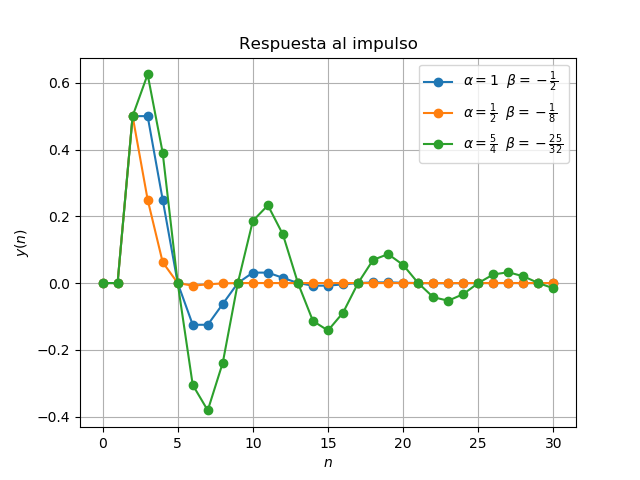
\includegraphics[width=\textwidth]{Imagenes/9-impulso.png}
\end{subfigure}
\begin{subfigure}{.7\textwidth}
\centering
	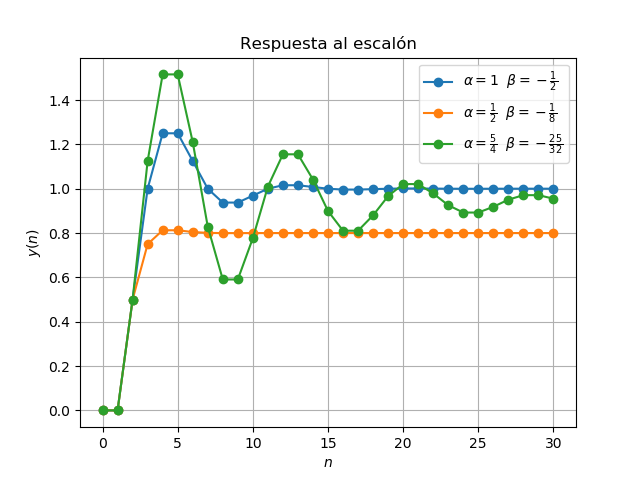
\includegraphics[width=\textwidth]{Imagenes/9-escalon.png}
\end{subfigure}
\end{figure}

\begin{center}
	\textcolor{red}{\textbf{Para estimar la respuesta el impulso en el caso de a...}}
\end{center}



\end{document}